% Options for packages loaded elsewhere
\PassOptionsToPackage{unicode}{hyperref}
\PassOptionsToPackage{hyphens}{url}
\documentclass[
]{book}
\usepackage{xcolor}
\usepackage{amsmath,amssymb}
\setcounter{secnumdepth}{-\maxdimen} % remove section numbering
\usepackage{iftex}
\ifPDFTeX
  \usepackage[T1]{fontenc}
  \usepackage[utf8]{inputenc}
  \usepackage{textcomp} % provide euro and other symbols
\else % if luatex or xetex
  \usepackage{unicode-math} % this also loads fontspec
  \defaultfontfeatures{Scale=MatchLowercase}
  \defaultfontfeatures[\rmfamily]{Ligatures=TeX,Scale=1}
\fi
\usepackage{lmodern}
\ifPDFTeX\else
  % xetex/luatex font selection
\fi
% Use upquote if available, for straight quotes in verbatim environments
\IfFileExists{upquote.sty}{\usepackage{upquote}}{}
\IfFileExists{microtype.sty}{% use microtype if available
  \usepackage[]{microtype}
  \UseMicrotypeSet[protrusion]{basicmath} % disable protrusion for tt fonts
}{}
\makeatletter
\@ifundefined{KOMAClassName}{% if non-KOMA class
  \IfFileExists{parskip.sty}{%
    \usepackage{parskip}
  }{% else
    \setlength{\parindent}{0pt}
    \setlength{\parskip}{6pt plus 2pt minus 1pt}}
}{% if KOMA class
  \KOMAoptions{parskip=half}}
\makeatother
\usepackage{graphicx}
\makeatletter
\newsavebox\pandoc@box
\newcommand*\pandocbounded[1]{% scales image to fit in text height/width
  \sbox\pandoc@box{#1}%
  \Gscale@div\@tempa{\textheight}{\dimexpr\ht\pandoc@box+\dp\pandoc@box\relax}%
  \Gscale@div\@tempb{\linewidth}{\wd\pandoc@box}%
  \ifdim\@tempb\p@<\@tempa\p@\let\@tempa\@tempb\fi% select the smaller of both
  \ifdim\@tempa\p@<\p@\scalebox{\@tempa}{\usebox\pandoc@box}%
  \else\usebox{\pandoc@box}%
  \fi%
}
% Set default figure placement to htbp
\def\fps@figure{htbp}
\makeatother
\ifLuaTeX
  \usepackage{luacolor}
  \usepackage[soul]{lua-ul}
\else
  \usepackage{soul}
\fi
\setlength{\emergencystretch}{3em} % prevent overfull lines
\providecommand{\tightlist}{%
  \setlength{\itemsep}{0pt}\setlength{\parskip}{0pt}}
\usepackage{bookmark}
\IfFileExists{xurl.sty}{\usepackage{xurl}}{} % add URL line breaks if available
\urlstyle{same}
\hypersetup{
  pdftitle={Manual de procedimentos para realização de grandes eventos do IIPC},
  hidelinks,
  pdfcreator={LaTeX via pandoc}}

\title{Manual de procedimentos para realização de grandes eventos do
IIPC}
\author{}
\date{}

\begin{document}
\frontmatter
\maketitle

{
\setcounter{tocdepth}{0}
\tableofcontents
}
\mainmatter
\textbf{IIPC}

\textbf{Manual de procedimentos para realização de grandes eventos do
IIPC}

\part{Manual}\label{manual}

\chapter{GRANDES EVENTOS}\label{grandes-eventos}

\begin{itemize}
\tightlist
\item
  Qualificação Docente
\item
  Encontro de Voluntários
\item
  Semana Docente
\item
  Congressos
\item
  Curso Projeciologia \& Reurbex
\item
  Celebrações instItucionais
\end{itemize}

\chapter{NÚCLEOS E EQUIPES}\label{nuxfacleos-e-equipes}

\begin{itemize}
\tightlist
\item
  Transmissão e Tecnologia da Informação
\end{itemize}

\chapter{OBJETIVO}\label{objetivo}

Organizar os diversos processos e fluxos de trabalho dos diferentes
Núcleos existentes para a otimização de cada um dos eventos nas
modalidades hibrida, \hl{presencial} ou à distância (online, síncrono).

\chapter{NÚCLEOS}\label{nuxfacleos}

\chapter{I -- TRANSMISSÃO E TECNOLOGIA DA
INFORMAÇÃO}\label{i-transmissuxe3o-e-tecnologia-da-informauxe7uxe3o}

\section{Objetivo}\label{objetivo-1}

Orientar os procedimentos para realização da transmissão dos Grandes
Eventos organizados pelo IIPC.

\section{Modalidade da transmissão}\label{modalidade-da-transmissuxe3o}

A depender do evento que está sendo organizado ele pode ser hibrido
(evento com interação online) ou online.

\section{Equipe}\label{equipe}

É importante ser previamente definida a equipe que será responsável pela
realização do Grande Evento. Caso seja na modalidade híbrido, as equipes
deverão ser formadas para acompanhamento de todo o processo, sendo
definido o número de voluntários e equipes de acordo com a proporção do
evento.

O IIPC deve definir um coordenador de transmissão nacional. Para cada
evento terá um epicentro que coordenará a transmissão do mesmo. Assim, o
epicentro coordenará as equipes, e dependendo da modalidade contará com
um epicentro que coordenará a equipe do presencial e outro epicentro que
coordenará a equipe do online.

\section{Tipos de Eventos}\label{tipos-de-eventos}

Os Grandes Eventos realizados pelo IIPC podem ser por meio de lives,
webinars, Cursos, talkshow e reuniões, como pré-evento e evento
principal.

\section{Plataforma e software
utilizado}\label{plataforma-e-software-utilizado}

A plataforma e software a ser utilizada vai depender do tipo de evento e
da modalidade escolhida.

As plataformas e software disponíveis mais comumente utilizadas e a
serem selecionadas para realização dos Grandes Eventos do IIPC são:
Zoom, Teams e StreamYard.

\subsection{StreamYard}\label{streamyard}

É um software que funciona como um estúdio virtual, onde você pode fazer
lives e transmiti-las através de redes sociais, até de forma simultânea,
em mais de uma plataforma ao mesmo tempo. O StreamYard é um software de
streaming em nuvem, usado na criação de conteúdos digitais ao vivo a
partir de um navegador. Com ele, é possível produzir lives, webinars,
apresentações e reuniões. Além disso, a ferramenta suporta a integração
com até oito plataformas de streaming e redes sociais para compartilhar
conteúdo de forma simultânea e em tempo real.

\subsection{Zoom}\label{zoom}

O Zoom é uma plataforma baseada em nuvem que possibilita realizar
videoconferências, cursos de treinamento online e outros tipos de
eventos \textbf{online.}

\subsection{Teams}\label{teams}

\section{Equipamentos}\label{equipamentos}

Os equipamentos necessários para a transmissão vai variar segundo a
modalidade: hibrido ou online.

Os equipamentos para uma transmissão presencial são:

\begin{itemize}
\tightlist
\item
  Equipamentos para captar imagem e som.
\item
  Um computador com conexão a internet e uma placa de captura.
\item
  Microfone profissional.
\item
  Microfone de lapela.
\item
  Switcher (mesa de corte) + controlador.
\item
  Mesa de som digital (sonorização).
\item
  iluminação profissional.
\item
  Televisão.
\item
  Celular.
\item
  Suporte para celular.
\item
  Suporte para câmera.
\end{itemize}

\chapter{\texorpdfstring{\textbf{Manual de procedimentos da
transmissão~}}{Manual de procedimentos da transmissão~}}\label{manual-de-procedimentos-da-transmissuxe3o}

\hl{Eventos somente online}~

Eventos híbridos~

\begin{itemize}
\tightlist
\item
  Equipamentos~
\end{itemize}

\begin{itemize}
\tightlist
\item
  Incluir fotos e etiquetar os equipamentos numerados~
\end{itemize}

\begin{itemize}
\tightlist
\item
  O que é utilizado no presencial e como?~
\end{itemize}

\begin{itemize}
\tightlist
\item
  {[}GABRIEL{]} Celular para filmagens do salão (iphone 8)~
\end{itemize}

\begin{itemize}
\tightlist
\item
  {[}ADQUIRIDO{]} Tripé para o celular de filmagens do salão~
\end{itemize}

\begin{itemize}
\tightlist
\item
  {[}WELTON{]} Celular para filmagens das perguntas (Samsung s9)~
\end{itemize}

\begin{itemize}
\tightlist
\item
  {[}A ADQUIRIR{]} Suporte de mão para o celular volante~
\end{itemize}

\begin{itemize}
\tightlist
\item
  {[}WELTON{]} Power bank para o celular de perguntas~
\end{itemize}

\begin{itemize}
\tightlist
\item
  {[}ADQUIRIDO{]} Computador desktop com 3 monitores (2 + 1 espelhado)~
\end{itemize}

\begin{itemize}
\tightlist
\item
  {[}ADQUIRIDO{]} Teclado e mouse para o desktop~
\end{itemize}

\begin{itemize}
\tightlist
\item
  {[}ADQUIRIDO{]} Projetor~
\end{itemize}

\begin{itemize}
\tightlist
\item
  {[}A ADQUIRIR{]} Passador de slides~
\end{itemize}

\begin{itemize}
\tightlist
\item
  {[}ADQUIRIDO{]} Espalhador HDMI (1 entrada = 4 saídas)~
\end{itemize}

\begin{itemize}
\tightlist
\item
  {[}ADQUIRIDO{]} Monitor espelho do projetor (conectado ao computador)~
\end{itemize}

\begin{itemize}
\tightlist
\item
  {[}ADQUIRIDO{]} Microfones sem fio (4)~
\end{itemize}

\begin{itemize}
\tightlist
\item
  {[}ADQUIRIDO{]} Mesa de som amplificada com bluetooth~
\end{itemize}

\begin{itemize}
\tightlist
\item
  {[}ADQUIRIDO{]} Receptor Bluetooth~
\end{itemize}

\begin{itemize}
\tightlist
\item
  {[}DO GABRIEL{]} Tripé da câmera principal~
\end{itemize}

\begin{itemize}
\tightlist
\item
  {[}ADQUIRIDO{]} Câmera principal~
\end{itemize}

\begin{itemize}
\tightlist
\item
  {[}ADQUIRIDO{]} Lente com bastante zoom~
\end{itemize}

\begin{itemize}
\tightlist
\item
  {[}ADQUIRIDO{]} Cabo RCA x P2 e Cabo P2 e P10 duplo (pelo menos 5m)~~
\end{itemize}

\begin{itemize}
\tightlist
\item
  {[}ADQUIRIDO{]} Extensão elétrica de diversos tamanhos~
\end{itemize}

\begin{itemize}
\tightlist
\item
  {[}A ADQUIRIR{]} Tablado para câmera e operador
\end{itemize}

\begin{itemize}
\tightlist
\item
  {[}A ADQUIRIR{]} Adaptadores DVI---HDMI~
\end{itemize}

\begin{itemize}
\tightlist
\item
  {[}A ADQUIRIR{]} Adaptador HDMI e VGA~
\end{itemize}

\begin{itemize}
\tightlist
\item
  {[}A ADQUIRIR{]} Monitores de palco (TV 42 polegadas)~
\end{itemize}

\begin{itemize}
\tightlist
\item
  {[}ADQUIRIDO{]} Cabo USB da câmera principal (com extensor USB)~
\end{itemize}

\begin{itemize}
\tightlist
\item
  {[}ADQUIRIDO{]} Nobreak~
\end{itemize}

\begin{itemize}
\tightlist
\item
  {[}INCERTO{]} Tripé para caixa de som?~
\end{itemize}

\begin{itemize}
\tightlist
\item
  {[}INCERTO{]} Caixa de som (Ribeirão Preto com amplificador)~
\end{itemize}

\section{\texorpdfstring{\textbf{Qual a melhor configuração de
posicionamento dos
equipamentos?~}}{Qual a melhor configuração de posicionamento dos equipamentos?~}}\label{qual-a-melhor-configurauxe7uxe3o-de-posicionamento-dos-equipamentos}

\begin{itemize}
\tightlist
\item
  Microfone de perguntas
\end{itemize}

\begin{quote}
Os microfones de perguntas podem ser opcionalmente fixo ou volante, a
depender do número de voluntários da equipe e da expertise dos mesmos.

No entanto, considerando que não temos câmera de alta qualidade e com
controle remoto, o microfone fixo para perguntas ainda é a nossa melhor
opção para os grandes eventos.
\end{quote}

\begin{itemize}
\tightlist
\item
  Monitor de palco
\end{itemize}

No mínimo devemos ter um monitor de palco. Caso o número de palestrantes
seja maior que cinco ou o espaço de palco seja extenso, podem ser
utilizados dois ou mais monitores de palco.

É importante ter na mesa de transmissão um monitor espelhado para o
monitor de palco.~

\begin{itemize}
\tightlist
\item
  Layout de conexão dos conectores.~
\end{itemize}

Antecedendo ao evento deve ser definido o esquema de conexões da
transmissão, com o esboço para que a equipe de transmissão possa
acompanhar o processo de instalação.

\begin{itemize}
\tightlist
\item
  Tripé da câmera principal
\end{itemize}

O posicionamento do tripé da câmera principal vai depender do tipo de
evento e do layout da sala, sendo preferencialmente numa altura mais
elevada.~

\begin{itemize}
\tightlist
\item
  \textbf{Papéis~da equipe de transmissão}
\end{itemize}

\begin{itemize}
\item
  Epicentro do evento~
\item
  Epicentro do presencial~
\end{itemize}

\begin{itemize}
\tightlist
\item
  Epicentro do online~
\end{itemize}

\begin{itemize}
\tightlist
\item
  \textbf{Processos e fluxos de trabalho~}
\end{itemize}

\begin{itemize}
\tightlist
\item
  Construção das planilhas~
\end{itemize}

Equipe -- construir uma planilha definindo as equipes, função e horários
de trabalho.

\begin{itemize}
\tightlist
\item
  Uso das pastas de apresentações e divulgações
\end{itemize}

\begin{quote}
A equipe de transmissão deve receber com antecedência as planilhas com
os materiais a serem divulgados durante o evento, assim como o roteiro
para orientação dos trabalhos.
\end{quote}

\begin{itemize}
\tightlist
\item
  Etiquetagem dos equipamentos~
\end{itemize}

Cada microfone é etiquetado com uma cor de referência, que é a mesma da
mesa de controle.

Computador com telas conectadas para: retroprojetor para apresentações
gerais; retroprojeto apresentando as pessoas do online para o
presencial; monitor para comunicação com equipe online e gerenciamento
dos materiais. ~

\hl{PARAMOS AQUI}

\begin{itemize}
\tightlist
\item
  Melhores práticas~
\end{itemize}

\begin{itemize}
\tightlist
\item
  A proximidade do monitor com o professor é fundamental para criar o
  rapport com o aluno online. (necessário ver o branco do olho).~
\end{itemize}

\begin{itemize}
\tightlist
\item
  Incluir diagramas de exemplo (ou captura de vídeo de algum evento).~
\end{itemize}

\begin{itemize}
\tightlist
\item
  Enquadramento utilizado na câmera principal deve ser bem apertado, bem
  próximo de quem está falando, para permitir uma boa experiência e
  conexão de quem está online.~
\end{itemize}

\begin{itemize}
\tightlist
\item
  Incluir diagramas de exemplo (ou captura de vídeo de algum evento).~
\end{itemize}

\begin{itemize}
\tightlist
\item
  Projetor: dependendo do evento tem que ser alugado~
\end{itemize}

\chapter{Como fazer uma transmissão ao vivo
(presencial)}\label{como-fazer-uma-transmissuxe3o-ao-vivo-presencial}

Estabeleça um objetivo.

Planeje o conteúdo.

Escolha os equipamentos.

Monte o cenário.

Cuide da iluminação.

Use equipamentos de captação de áudio.

Tenha uma boa conexão de internet.

Faça testes antes de iniciar a~transmissão.

Quadro com quantidade, especificação, próprio ou para aluguel

Como proceder em caso de contratação de empresa para aluguel de
equipamento.

Transmissão presencial em espaço próprio do IIPC e em local alugado
(como hotel).

Desafios e soluções

Dicas de otimizações

Prazo para cada etapa

Responsabilidades -- equipes

Iniciativas de segurança: redundância;

Situações exemplificadoras a partir das experiências vivenciadas

\chapter{Cronograma para elaboração do Manual de
Procedimentos}\label{cronograma-para-elaborauxe7uxe3o-do-manual-de-procedimentos}

\part{ANOTAÇÕES DE ANA CERES}\label{anotauxe7uxf5es-de-ana-ceres}

===========================================================

\textbf{7 ago 2024}

Seguem algumas orientações e preparativos para o curso:

1. Procure um ambiente reservado na sua residência para acompanhar todo
o curso sem interrupções externas, a fim de manter a concentração e a
conexão com a equipe extrafísica de amparadores.

2. Se organize com papel e caneta à mão para as suas anotações pessoais.

3. Por questão de parassegurança, não é indicado participar do evento em
trânsito (dirigindo ou como passageiro) e em locais públicos (ônibus,
hospital, praça pública, lanchonete, etc).

4. Mantenha a câmera aberta e o microfone fechado durante a explanação.
A qualquer momento você poderá abrir o microfone e trazer suas dúvidas e
contribuições, para isso clique na mãozinha ou levante mão para que os
professores possam lhe chamar.

5. Providencie um local com bom acesso à internet.

6. A sala será aberta às 8h45 e o curso iniciará pontualmente às 9h.
Procure entrar com antecedência para testar o microfone e para evitar
problemas técnicos.

7. O curso será realizado na plataforma Zoom. Certifique-se de tê-lo
instalado em seu computador ou celular previamente.

O link de acesso ao zoom será enviado aqui no grupo.

Orientação para o aluno online

=================================================================

\textbf{8 ago 2024}

\textbf{Monitoria Transmissão I Congresso de Conscienciologia}

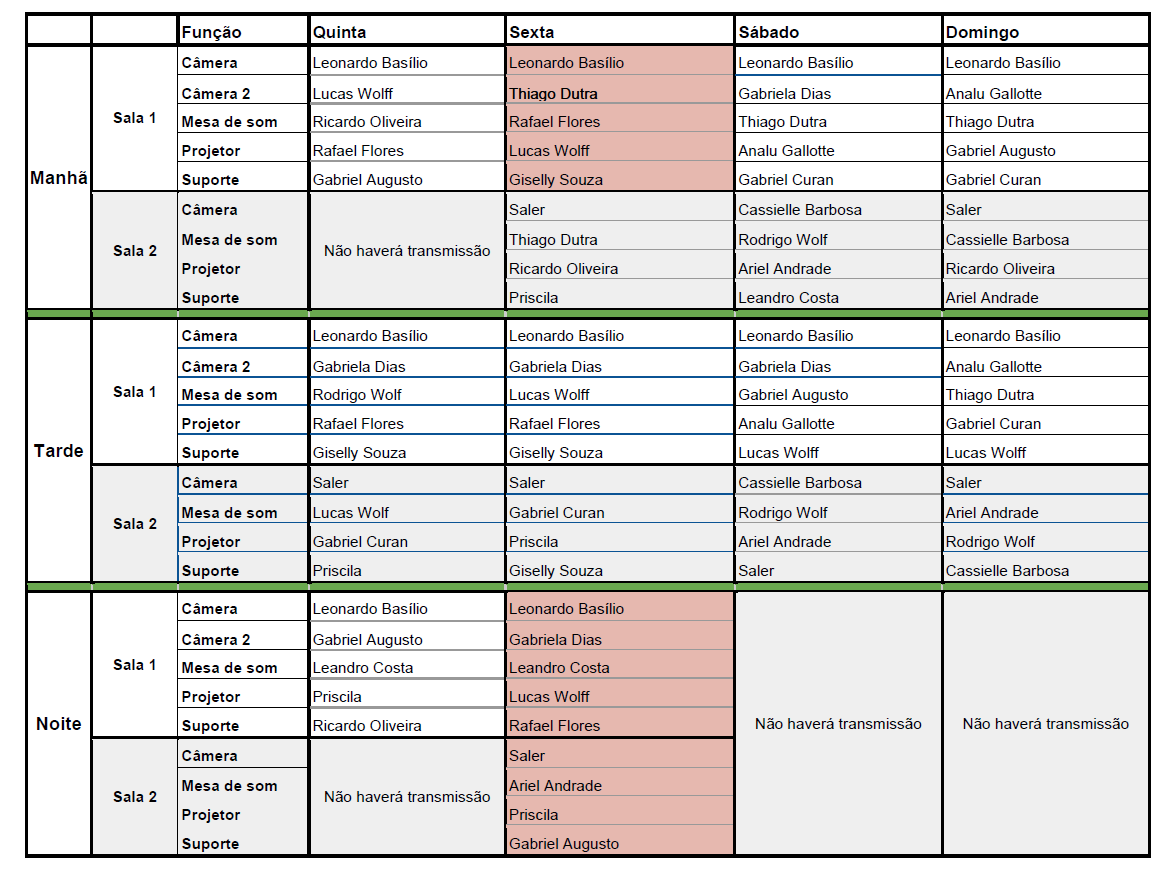
\includegraphics[width=5.90556in,height=4.4569in]{./media/image1.png}

\textbf{Checklist - Função projetor}

\begin{itemize}
\item
  \textbf{Slides} - conferir se todos estão numerados de acordo com a
  sequência de apresentação do turno;
\item
  \textbf{Powerpoint} - Conferir se todas as apresentações estão em
  formato powerpoint;
\item
  \textbf{Apresentação} - Conferir o modo de apresentação testando;
\item
  \textbf{Zoom-} Compartilhamento com Zoom -- testar;
\item
  \textbf{Som} - Conferir se há vídeos ou áudios no slade e passar a
  informação para a mesa de som;
\item
  \textbf{Vídeo} - Observar no documento do cerimonial se há algum vídeo
  preparar a apresentação e passar a informação para a mesa de som;
\item
  \textbf{Sorteio} - Observar no documento do cerimonial se há sorteio.
\item
  \textbf{Transmissão com Palestrantes online}-
\end{itemize}

\begin{itemize}
\item
  Compartilhar o slide do professor;
\item
  Passar o controle do slide para o professor online;
\item
  Deixar 2 projetores com a imagem do slade e outro com o a imagem do
  professor; (para isso é necessário mais um computador conectado ao
  zoom)
\end{itemize}

\textbf{Checklist - Função Mesa de som}

\begin{itemize}
\item
  \textbf{Pilhas} -- Ao iniciar o turno, conferir se todas as pilhas dos
  microfones estão carregadas; retirar pilhas descarregadas ou com carga
  baixa dos microfones e por pra carregar;
\item
  \textbf{Mesa de som} - Controlar som dos microfones presenciais e do
  som vindo do computador.
\item
  \textbf{Programação} - Conferir com a monitoria dos slides se há
  vídeos a serem
\item
  \textbf{Som Ambiente} - Deixar no começo e nos intervalos do evento
  som de fundo com da playlist pré-selecionada. (Em parceria com
  monitoria dos slides)
\item
  \textbf{Slides} - Conferir se os slides estão numerados de acordo com
  a sequência de apresentação do turno;
\end{itemize}

\textbf{Checklist -- Suporte}

\begin{itemize}
\item
  \textbf{Atenção} - Ficar atendo às demandas da transmissão;
\item
  \textbf{Apoio} - Ficar na função dos colegas escalados em caso de
  necessidade;
\end{itemize}

\textbf{Checklist -- Câmera}

\begin{itemize}
\item
  \textbf{Foco} - Filmar todo o evento revezando câmeras de palco e
  perguntas;
\item
  \textbf{Gravar} - Fazer a gravação de todos os períodos do evento na
  máquina;
\end{itemize}

==============================================

12 ago 2024

São as informações sem as quais o IIPCNET não aceita agendar o evento. É
importante também que o release e a arte tenham passado pela avaliação
do Técnico Científico antes, para evitar que o link~saia~com~erros.

\url{https://1drv.ms/w/c/ca868f0c70d8b973/Eab1KCyztY1CuSGbkljkKY0BTRhEwPmO1bCWeKGHpdZ86g?e=7VO2eL}

Checklist para a criação e agendamento de eventos:

Título do Curso ou Evento;

Tipo: Presencial ou online;

Tema;

Início data e hora;

Fechamento do evento (data e horário);

Término (data e horário, geralmente o mesmo do fechamento);

Dias da semana;

Datas das aulas;

Horário (dia da semana com horário de início e término pela manhã,
horário de intervalo e início e término à tarde ou noite);

Localidade: (IIPC SEDE ou outro);

Local (cidade);

Endereço;

Plataforma de Publicação: Woocommerce para pagos e Sympla para
gratuitos;

No de vagas;

No de alunos previstos;

Ticket médio previsto;

Executivo;

Professor P1;

Professor P2;

Monitor;

Para a solicitação do link é necessário anexar:

Release aprovado pelo Técnico Científico;

Arte aprovada pelo Técnico~Científico.

\textbf{Referências}

\begin{enumerate}
\def\labelenumi{(\arabic{enumi})}
\tightlist
\item
  https://rockcontent.com/br/blog/streamyard/
\end{enumerate}

\backmatter
\end{document}
